\documentclass[11pt]{amsart}
\usepackage{geometry}                % See geometry.pdf to learn the layout options. There are lots.
\geometry{a4paper}                   % ... or a4paper or a5paper or ...
%\geometry{landscape}                % Activate for for rotated page geometry
\usepackage[parfill]{parskip}    % Activate to begin paragraphs with an empty line rather than an indent
\usepackage{enumitem}
\usepackage{graphicx}
\usepackage{amssymb}
\usepackage{amsmath}
\usepackage{cancel}
\usepackage{epstopdf}
\DeclareGraphicsRule{.tif}{png}{.png}{`convert #1 `dirname #1`/`basename #1 .tif`.png}
\usepackage{breqn}
\usepackage{float}
\usepackage{breqn}

\title{Econ 210C Problem Set \# 4}
\author{Minki Kim}
%\date{}                                           % Activate to display a given date or no date

\begin{document}




\maketitle

\section{Labor supply problem}
An individual with time-separable utility solves the following maximization problem: 
\begin{equation*}
\mathcal{L} = \sum_{t=0}^{\infty} \beta^t \bigg( \log C_t + \log (1-L_t)  + \lambda_t  \left(  w_t L_t - C_t \right) \bigg)
\end{equation*}
The first order conditions of the individual are: 
\begin{align*}
\frac{1}{C_t} &= \lambda_t  \\
\lambda_t w_t &= \frac{1}{1-L_t} 
\end{align*}
On the other hand, an individiual with non-separable preferences solves the following dynamic maximization problem :
\begin{equation*}
\mathcal{L} = \sum_{t=0}^{\infty} \beta^t \bigg( \log C_t + \log\left( 1 - 0.5 \left[ L_t + L_{t-1} \right] \right) + \lambda_t  \left(  w_t L_t - C_t \right)  \bigg)
\end{equation*}
The first order conditions for this individual are: 
\begin{gather*}
\frac{1}{C_t} = \lambda_t  \\
\lambda_t w_t = \frac{0.5}{1 - 0.5 \left( L_t + L_{t-1} \right)} + \beta \frac{0.5}{1 - 0.5 \left( L_{t+1} + L_t \right)}
\end{gather*}
\begin{enumerate}[label=(\alph*)]
	\item I assume that there is no means for individuals to save in the economy. Hence, the budget constraint $w_t L_t = C_t$ is satisfied every period. Then, for an individual with separable utility, labor supply is just 
	\begin{equation*}
	L_t = \frac{1}{2}
	\end{equation*}
	Therefore, labor supply does not respond to shocks in this case. Now consider the labor supply for an individual with non-separable preferences. Labor supply for those individuals is characterized by the following equation:
	\begin{equation*}
	\frac{w_t}{C_t}  = \frac{0.5}{1 - 0.5 \left( L_t + L_{t-1} \right)} + \beta \frac{0.5}{1 - 0.5 \left( L_{t+1} + L_t \right)}
	\end{equation*}
	When the positive shock is expected to hit the economy in period $t$, the individual can adjust her labor supply not just in period $t$, but period $t-1$ and $t+1$. For instance, in the wake of negative shock, the individual can choose to work less in period $t$ (when the negative shock is in effect) and work more in the adjacent two periods. Therefore, compared to the case when the utility was separable, labor supply changes are larger to the same shock. 
	
	\item Since $L_t = \frac{1}{2}$ for the separable preferences, labor supply is perfectly inelastic ($\varepsilon_{L,w} = 0$). One would generate higher value of labor supply elasticity by introducing non-separability to preferences. 
\end{enumerate}
\section{Demand shock}
\begin{enumerate}[label=(\alph*)]
	\item A representative consumer solves the following utility maximization problem: 
	\begin{equation*}
	\mathcal{L} = \sum_{t=0}^{\infty} \beta^t \left[ \log C_t - \nu_t \frac{L_t^{1 +\chi}}{1+\chi} + \lambda_t \left( W_t L_t + (P_t + d_t) K_t + \Pi_t - C_t - P_t K_{t+1} \right) \right]
	\end{equation*}
	The first order conditions are: 
	\begin{align*}
	\frac{1}{C_t} &= \lambda_t \\
	\nu_t L_t^\chi &= \lambda_t W_t \\
	\lambda_t P_t &= \beta \mathbb{E}_t \lambda_{t+1} \left(  P_{t+1} + d_{t+1} \right)  \\
	P_t K_{t+1} + C_t & = W_t L_t + (P_t + d_t) K_t + \Pi_t
	\end{align*}
	
	\item Suppose the representative consumer reduces one unit of consumption today and invest those forgone amount of consumption into capital. By giving up one unit of consumption today, the consumer incurs a marginal loss in utility: $\lambda_t$. 
	
	However, the consumer now can use increased amount of capital the next period. Additional amount of capital generates additional amount of dividend net the cost paid to purchase the additional capital in period $t$, which is captured by $\frac{d_{t+1}}{P_t}$, which can be converted to utility term by multiplying $\lambda_{t+1}$. On top of this, the consumer can enjoy a capital gain or incur a capital loss depending on how the price of capital changes from $t$ to $t+1$. This is captured by $\frac{P_{t+1}}{P_t}$. Finally, all these gains are discounted by $\beta$ because they are realized in period $t+1$. In conclusion, we get 
	\begin{equation*}
	\lambda_t = \beta \mathbb{E}_t \frac{\lambda_{t+1} (P_{t+1} + d_t)}{P_t}
	\end{equation*}
	
	\item
	\item
	\item
\end{enumerate}
\section{Business cycle and external returns to scale}
\begin{enumerate}[label=(\alph*)]
	\item 
	\item
	\item
	\item
	\item
\end{enumerate}
\section{Problems from Romer}
\subsection{Problem 6.10}
\begin{enumerate}[label=(\alph*)]
	\item Using the given three equations, it is easy to get the closed form solution for $p, p^{*}$, and $y$. 
	\begin{align*}
	p & = \frac{f \phi m'}{1 - f + f\phi} \\
	p^{*} & = \frac{\phi m'}{1 - f + f\phi} \\
	y & = \frac{m' (1-f)}{1 - f + f\phi}
	\end{align*}
	\item The following figure summarizes the results
	\begin{figure}[H]
		\centering
		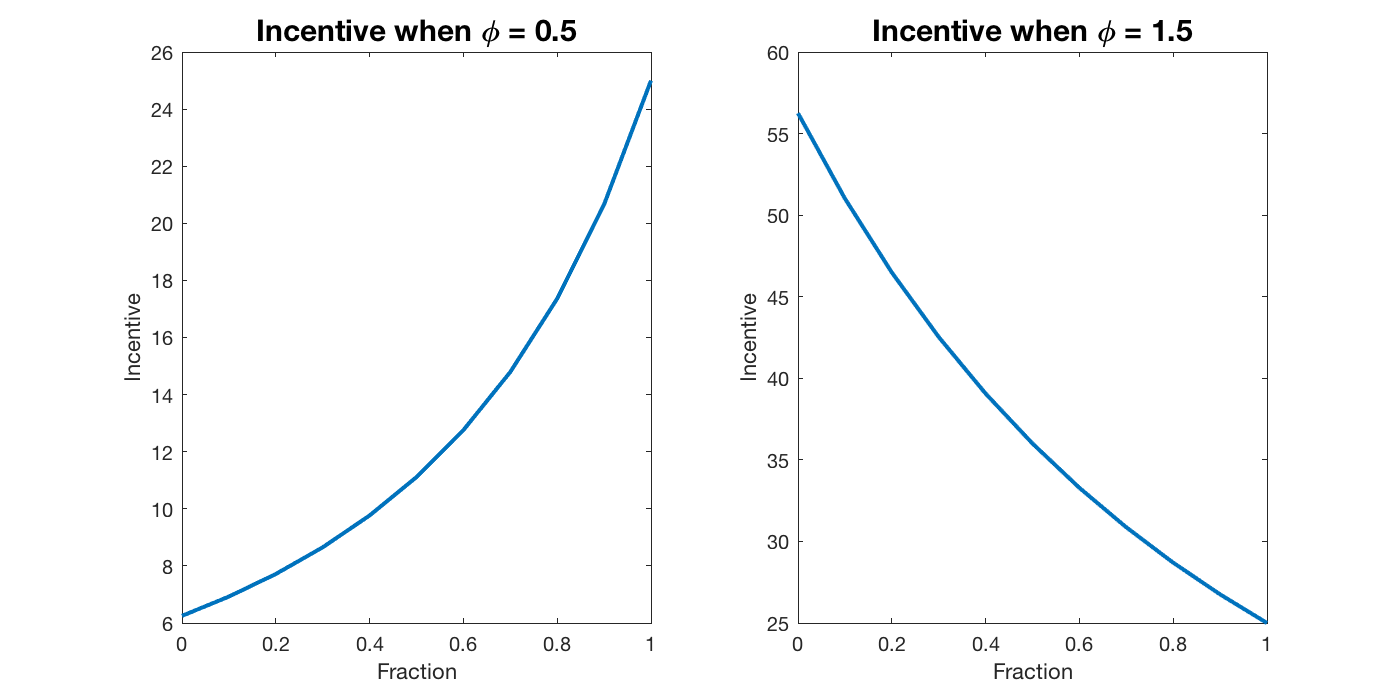
\includegraphics[width=0.85\textwidth]{611b}
		\caption{A firm's incentive to adjust its price}
	\end{figure}
	\item Whether a firm adjusts its price or not depends on the size of the menu cost, $Z$. Assume that $\phi <1$. Now suppose the menu cost is very low, lower than the incentive of a firm when no other firm is adjusting their prices. In this case, all firms adjusting their prices can be a Nash equilibrium. 
	
	Suppose, on the other hand, the case when the menu cost is really high, higher than the incentive of a firm when all the other firms are adjusting their prices. In this case, no price adjustment is the only Nash equilibrium. 
	
	Now suppose that the size of the menu cost lies somewhere between the above two extremes. Specifically, say that $Z = K p^{*} (f)$ for some $f$. Then, a fraction $f$ of the firms adjusting their prices is the only Nash equilibrium, because for $f' \neq f$ some firms have incentives to deviate from adjusting (not adjusting) prices. 
\end{enumerate}
\subsection{Problem 6.11}
\begin{enumerate}[label = (\alph*)]
	\item If the firm does not adjust its price and stays at $r^{*}(y_0)$ level, its profit is $\pi \left( y_1, r^{*}(y_0)  \right)$. On the other hand, if the firm choose to adjust its price to the optimal level for $y_1$, its profit is $\pi \left( y_1, r^{*}(y_1)  \right)$ The difference between these two is a potential gain from adjusting the price, so can be interpreted as the incentive to adjust its price. 
	\item Second-order Taylor approximation of $G = \pi \left( y_1, r^{*}(y_1)  \right) - \pi \left( y_1, r^{*}(y_0)  \right)$ is: 
	
	\begin{align*}
	G &= \pi \left( y_1, r^{*}(y_1)  \right) - \pi \left( y_1, r^{*}(y_0)  \right) \\
	 & \simeq 
	\end{align*}
	\item 
\end{enumerate}
\subsection{Problem 6.12}

\end{document}
